\chapter{Algebraic Review}
\label{ch:algebra}

In this chapter we shall discuss algebraic theoretical background that grounds cryptography schemes.


\section{Basic structures}
% groups, quotient groups, cosets, rings, quotient rings, fields

\begin{definition}[Group]

A non-empty set G is called a group under the operation $*$, if it satisfies the following three axioms:

\begin{alineas}
    \item  (Closure) G is closed under $*$, i.e, for all $a,b\in G$, the result $a*b$ is also in $G$;
    \item (Associativity) $(a* b)* c = a\times (b*c)$, for all $a,b,c\in G$;
    \item (Existence of identity) There exists $e\in G$ such that $a*e=e*a=a$ for all $a\in G$;
    
    We shall denote the group as $(G,*)$. If, in addition to the above axioms, the group also satisfies the next property, it is called an \textbf{abelian group}.
    
    \item (Commutativity) For all $a,b\in G$, $a*b=b*a$.
\end{alineas}
\end{definition}

A set $R$ is called a (commutative) \textbf{Ring} if it has two operations: addition ($+$) and multiplication ($\times$) satisfying the following properties:

\begin{itemize}
    \item $R$ is an abelian group under addition
    \item (multiplicative associativity) $(a\times b)\times c = a\times (b\times c)$, for all $a,~b,~c\in R$ ;
    \item (distributivity) $a\times (b+c)=a\times b + a\times c$ for all $a,~b,~c\in R$;
    \item (multiplicative commutativity) $a\times b=b\times a$ for all $a,~b\in R$;
    \item (multiplicative inverse) There exists an element $1$, such that, $1\times a = a\times 1 = a,$ for all $a\in R$.
\end{itemize}

\section{Polynomial Rings}

\section{Cyclotomic polynomials and its properties}

In this section, we define and review some properties of cyclotomic polynomials, which will play a central role in the homomorphic cryptography setup.

\begin{definition}[Roots of unity] The $n^{th}$ roots of unity are the solution set of the equation $x^n-1=0$ in the field of complex number $\mathbb C$:
$$\sqrt[n]1=\{\zeta_n^k;k=0,1,\ldots,n-1\},$$
where\footnote{In Euler's notation $\exp{(i\theta)}=\cos\theta+i\cdot\sin\theta$} $\zeta_n=\exp{(2\pi i/n)}$
\end{definition}
In the complex plane, this roots are distributed over the unitary circumference and equally separated by an angle of $2\pi/n$. Figure \ref{fig:roots_of_unity} show the example of the $8^{th}$ roots of unity.

\begin{figure}[!htb]
    \centering
    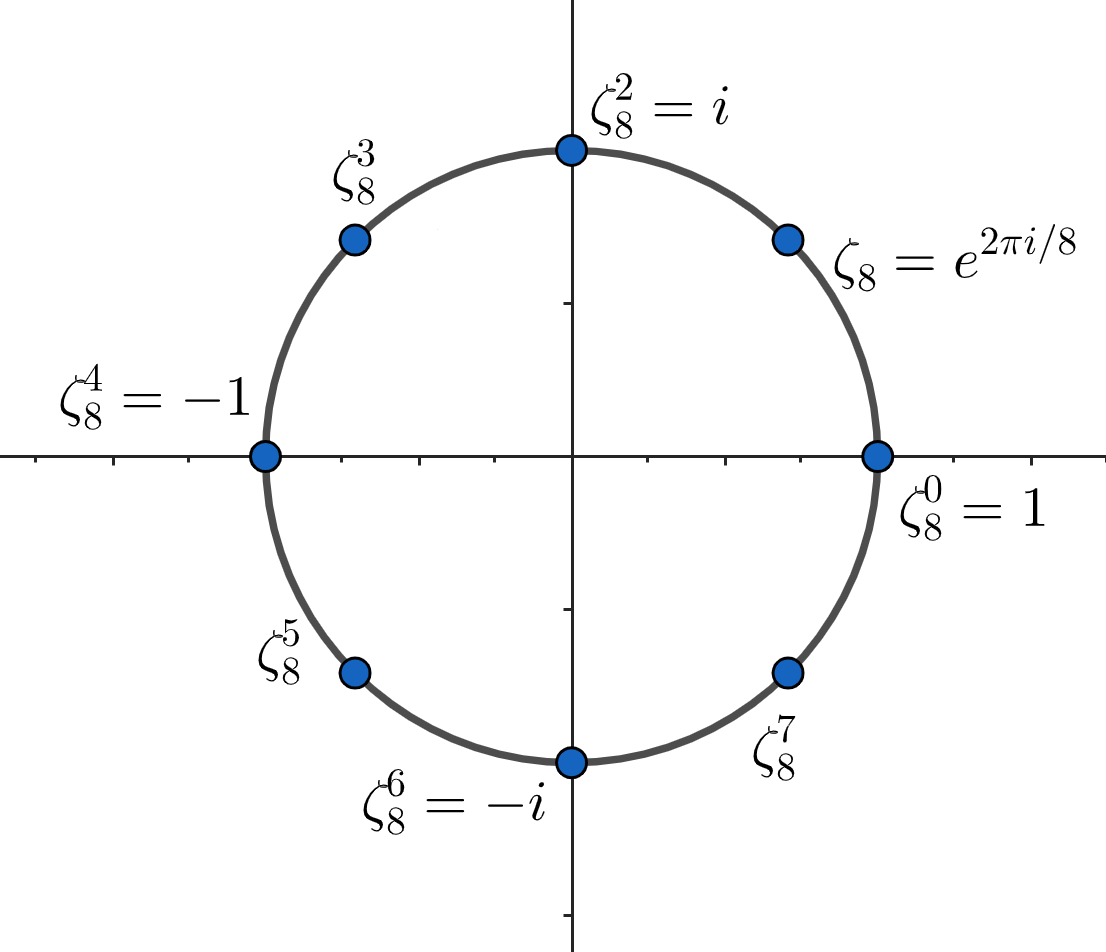
\includegraphics[scale=0.4]{files/figures/roots_of_unity.png}
    \caption{$8^{th}$ roots of unity}
    \label{fig:roots_of_unity}
\end{figure}

\begin{definition}[Primitive roots of unity]\cite{brilliant}
The $n^{th}$ primitive roots of unity are:
$$\{\zeta \in \mathbb C;\zeta^n=1\text{ and }\zeta^k\neq1,\forall ~ k<n \},$$
for positive integers $k$. They are the subset of $n^{th}$ roots of unity which are not $k^{th}$ roots of unity, for all $k<n$. They can be alternatively defined as:
$$\{\zeta_n^k;1\leq k \leq n,\gcd(k,n)=1\}$$
\end{definition}
From the Figure \ref{fig:roots_of_unity} example, the $8^{th}$ primitive roots of unity are $\zeta_8,\zeta_8^3,\zeta_8^5,\zeta_8^7$.
% Indeed, $\zeta_n^k=\exp(2k\pi i/n)$ will be equal to $1$ if, and only if the exponent is an integer multiple of $2\pi i$, which is not the case when $\gcd(k,n)=1$, since $k/n$
% tmp\cite{brilliant}

\begin{definition}[Cyclotomic polynomial] \label{def:cyclo}The \textit{$n$-th cyclotomical polynomial} is defined as:
\begin{align*}
    \Phi_n(x) = \prod_{\substack{1\leq k \leq n\\ \gcd(k,n)=1}}^{n}(x-\zeta_n^k)
\end{align*}
\end{definition}

Notice that its roots are the $n^{th}$ primitive roots of unity.

Using the definition, we can derive some cyclotomical polynomials, for example $\Phi_1(x)=x-1$ trivially, and $\Phi_2(x)=x+1$, since from the $2^{nd}$ roots of unity $-1$ and $+1$, only $-1$ are primitive ones.

The $3^{rd}$ primitive roots of are $\zeta_3^1$ and $\zeta_3^2=\overline{\zeta_3^1}$, then:
\begin{align}
    \Phi_3(x)&=(x-\zeta_3^1)(x-\zeta_3^2)\nonumber\\
    &=x^2-x(\zeta_3^1+\zeta_3^2)+\zeta_3^1\zeta_3^2\nonumber\\
    &=x^2-x(\zeta_3^1+\overline{\zeta_3^1})+e^{2\pi i(1+2)/3}\label{eq:zeta3}\nonumber\\
    &=x^2-x(2\cdot\cos(2\pi/3))+e^{2\pi i}\\
    &=x^2+x\left(2\cdot \frac12\right)+1\nonumber\\
    &=x^2+x+1\nonumber
\end{align}

The equality (1) holds due to the sum of complex conjugates being equal to two times the real part since we cancel out the imaginary terms.

\begin{theorem} \label{teoremaco}For all positive integers $n$ we have:
$$\displaystyle x^n-1=\prod_{d|n}\Phi_d(x)$$
\end{theorem}

The above theorem provides a analytical formula to recursively generate the cyclotomic polynomials:
$$\displaystyle\Phi_n(x)=\dfrac{x^n-1}{\displaystyle\prod_{\substack{d|n\\d\neq n}}\Phi_d(x)}$$

We can use it to derive simpler, and non-recursive expressions for particular interesting cases:

\begin{corollary}[Prime Cyclotomical Polynomial]
If $p$ is a prime number, then:
$$\Phi_p(x)=x^{p-1}+x^{p-2}+\ldots+x+1$$
\end{corollary}

\begin{proof}
By the previous theorem, and the fact that the only $d<p$ satisfying $d|n$ is $d=1$:

$$\Phi_p(x)=\dfrac{x^p-1}{\displaystyle\prod_{\substack{d|p\\d\neq p}}\Phi_d(x)}=\dfrac{x^p-1}{\Phi_1(x)}=\dfrac{x^p-1}{x-1}$$

The polynomial division algorithm concludes that such a division actually results in what is claimed in the corollary.

An easy way to assert it, is by multiplying the divisor $x-1$ by $\displaystyle\sum_{i=0}^{p-1}x^i$ and checking if it is equal to $x^p-1$:
\begin{align*}
    (x-1)\left(\sum_{i=0}^{p-1}x^i\right)&=\sum_{i=0}^{p-1}x^{i+1}-\sum_{i=0}^{p-1}x^i\\
    &=\sum_{i=0}^{p-1}x^{i+1}-x^{i}\\
    &=x^{(p-1)+1}-x^{0}\\
    &=x^{p}-1
\end{align*}
\end{proof}
The following formula will be crucial to instantiate plaintext and cyphertext spaces in the encryption schemes.
\begin{corollary}[Power of Two Cyclotomic Polynomial]
If $M=2^n$, for a given positive integer $n$, then:
$$\Phi_M(x)=x^{M/2}+1$$
\end{corollary}
\begin{proof}
We'll proceed by strong induction in $n$ \cite{herstein1996abstract},  proving an equivalent statement\footnote{One can easily verify that $\dfrac{x^{M}-1}{x^{M/2}-1} = x^{M/2}+1$ using the polynomial division algorithm for example, or multiplying the divisor with the quotient}: 
\begin{equation}
\label{eq:phim}
    \Phi_{M_n}(x) = \dfrac{x^{M_n}-1}{x^{M_n/2}-1}
\end{equation}
We're denoting $2^n$ by $M_n$ to have a cleaner notation of nested exponents; hence $M_n/2=M_{n-1}$.

(Base case) For $n=1$, $\Phi_{M_1}(x)=\Phi(2)=x+1$, as we derived before. This is the LHS of \ref{eq:phim}. The RHS is $\frac{x^2-1}{x-1}=\frac{(x+1)(x-1)}{x-1}=x+1$, so the formula is valid in this case.

(Inductive Hypothesis) Assume that \ref{eq:phim} hold for $M_k$ for all $k<n$ positive integers.

(Inductive Step) Let's deduce that it also holds for $M_n$: By Theorem  \ref{teoremaco}, we have:
\begin{align*}
    \Phi_{M_n}(x) &= \dfrac{x^{M_n}-1}{\displaystyle\prod_{\substack{d|M_n\\d\neq M_n}}\Phi_d(x)}
\end{align*}
Notice that $\{d\in\mathbb{Z}^+;d|M_n\} = \{M_0,M_1,\ldots,M_{n-1}\}$, i.e., the divisors of $M_n$ are the powers of two with exponent less than $n$. Then our expression becomes:
$$\Phi_n(x) = \dfrac{x^{M_n}-1}{\Phi_{M_0}\Phi_{M_1}\ldots\Phi_{M_{n-1}}}$$
Using the inductive hypothesis we can rewrite the denominator as:
$$\Phi_{M_0}\Phi_{M_1}\ldots\Phi_{M_{n-1}}=$$



\end{proof}

\section{Lattices}

\section{LWE and RLWE}

\chapter{Homomorphic Encryption}

\section{Privacy Homomorphisms}

Assume we can represent the unencrypted data by an algebraic structure $\mathcal P= (S;f_1,\ldots,f_k)$, i.e., a set $S$ ported with the operations $f_1,\ldots,f_k$. We will further call this structure the plaintext space.

An alternative algebraic structure, the cyphertext space $\Cypher=(S',f'_1,\ldots,f'_k)$, is constructed to represent the encrypted data. To build a \textit{privacy homomorphism} \cite{Rivest1978},  one needs a decryption function $\phi:S'\to S$ and its inverse $\phi^{-1}:S\to S'$ satisfying the homomorphic property from $\Cypher$ do $\Plain$:
\begin{align}
    \label{privhom}
    f'_i(a,b,\ldots)&=c\Rightarrow\nonumber\\ f_i(\phi(a),\phi(b),\ldots)&=\phi(c),\text{ for } i=1,\ldots,k\\
    \text{with }a,b,&\ldots\in S'\nonumber
\end{align}
This means that for all available operations $f'_i$, its evaluation on encrypted elements must result in a value that, after decryption, corresponds to the same computation on the unencrypted domain.

An example of privacy homomorphism is the RSA cryptosystem \cite{rsa}, which uses $\Plain = (\Z_p;\times_p)$, the integers modulo $p$ with $p$ prime, and the multiplication modulo $p$. Setting $N=pq$, where $q$ is a large prime and choosing $e$ coprime with $(p-1)(q-1)$,  the cyphertext space as $(\Z_N;\times_N)$ and is connected with $\Plain$ through the encryption function:
\begin{align*}
    \phi^{-1}&:\Z_p\to\Z_N\\
    \phi^{-1}(x)&=x^e(\bmod N)
\end{align*}
Taking $x,y\in\Z_p$ and its encrypted versions $x'=\phi^{-1}(x),~y'=\phi^{-1}(y)$, we have:
\begin{align*}
    x'\times_N y'&= (x^e)(y^e)(\bmod N)\\
    &=(xy)^e(\bmod N),
\end{align*}
which is an encryption of $xy$. Then the multiplication satisfies property \ref{privhom}, showing that such a system is indeed a privacy homomorphism.

\subsection{Requirements and Limitations}
The following properties for $\Cypher,\phi$ and $\phi^{-1}$ are required by the authors:
\begin{alineas}
    \item for a given element $s\in S$, its encrypted version $\phi^{-1}(s)$ should not require much more storage space;
    \item $\phi$ and $\phi^{-1}$ should be easy to compute;
    \item the operations $f_i'$ should be efficiently computable in $\Cypher$;
    \item $\phi$ should not be vulnerable to the chosen plaintext attack;
    \item The operations of $\Cypher$ should not be sufficient to yield an efficient computation of $\phi$.
\end{alineas}

The last requirement forces a critical restriction on such morphisms: a comparison operator ``$\leq$'' can't be available in the cyphertext space, otherwise, no secure privacy homomorphism exists.

Take for example $\Plain = (\N;+,\leq)$ and $\Cypher = (W;+',\leq')$ for some $W$. A malicious party who has $\phi^{-1}(n)$, and wants to discover what $n\in\N$ generated such cyphertext can apply the following binary search strategy:
\begin{alineas}
\item compute $1'=\phi^{-1}(1)$;
\item compute $2'=1'+'1'$, then $4'=2'+'2'$;
\item continue until finding $k$, such that $\phi^{-1}(n)\leq'(2^k)'=\phi^{-1}(2^k)$
\item knowing that $n\in[2^{k-1},2^{k}]$, compute an encryption of the interval midpoint $\phi^{-1}(m)=\phi^{-1}(2^{k-1}-2^{k-2})$;
\item homomorphically compare $\phi^{-1}(n)\leq'\phi^{-1}(2^{k-1})+'\phi^{-1}(m)$;
\item repeat the last two steps properly redefining the interval until getting $n$ exactly.
\end{alineas}
This is an efficient $O(\log n)$ algorithm to compute the decryption function $\phi$, using the operations in $\Cypher$ and the ability to generate encryptions of arbitrary constants (such as $1$ and $m$ in the above example).

The article finishes with the authors pondering if such an approach with all required security restrictions could be worthwhile in practice and what algebraic structures $\Plain$ would provide usefuls privacy homomorphisms.
% \section{First Generation Fully Homomorphic schemes}
% \begin{alineas}
% \item somewhat/fully homomorphic
% \item bootstrapping
% \item integer scheme
% \item caveats and implementation paper
% \end{alineas}

\section{Fully Homomorphic Encryption}
\section{Gentry's work}


\subsection{BFV and BGV schemes (integers)}

\begin{alineas}
\item describe BFV primitives (codec/ring)
\item encrypt/decrypt
\item relinelization
\item BGV differences
\end{alineas}

\subsection{CKKS scheme (complex numbers)}

- brief description about fixed point arithmetic?
- the complex map 
- 
\subsection{Approximate Bootstrapping}

\chapter{Private Logistic Regression}
\section{Statistical Review}
\section{Homomorphic Training}
\section{Data Applications}


\label{ch:algebra}

